\documentclass{report}
\usepackage{graphicx}
\begin{document}

\title{ETERNITY: FUNCTIONS}
\author{Wenshu Li\\Student ID: 40203982}
\date{}
\maketitle

\makeatletter
\let\thetitle\@title
\let\theauthor\@author
\let\thedate\@date
\makeatother





% This will generate a table of contents
\tableofcontents
\newpage
\section{Introduction}
\subsection{Discription}
In mathematics, the gamma function is one commonly used extension of the factorial function to complex numbers. The gamma function is defined for all complex numbers except the non-positive integers. For any positive integer n, 
\\$$\Gamma \left ( n\right ) = \left ( n-1 \right )!$$ 
\\ Derived by Daniel Bernoulli, for complex numbers with a positive real part, the gamma function is defined via a convergent improper integral:
\\$$\Gamma \left ( n\right ) = \int_{0}^{\infty} x^{z-1} e^{-x}\mathrm{d}x,  \Re\left ( z \right )>0$$
\begin{figure}[h]
\caption{Gamma function}
\centering
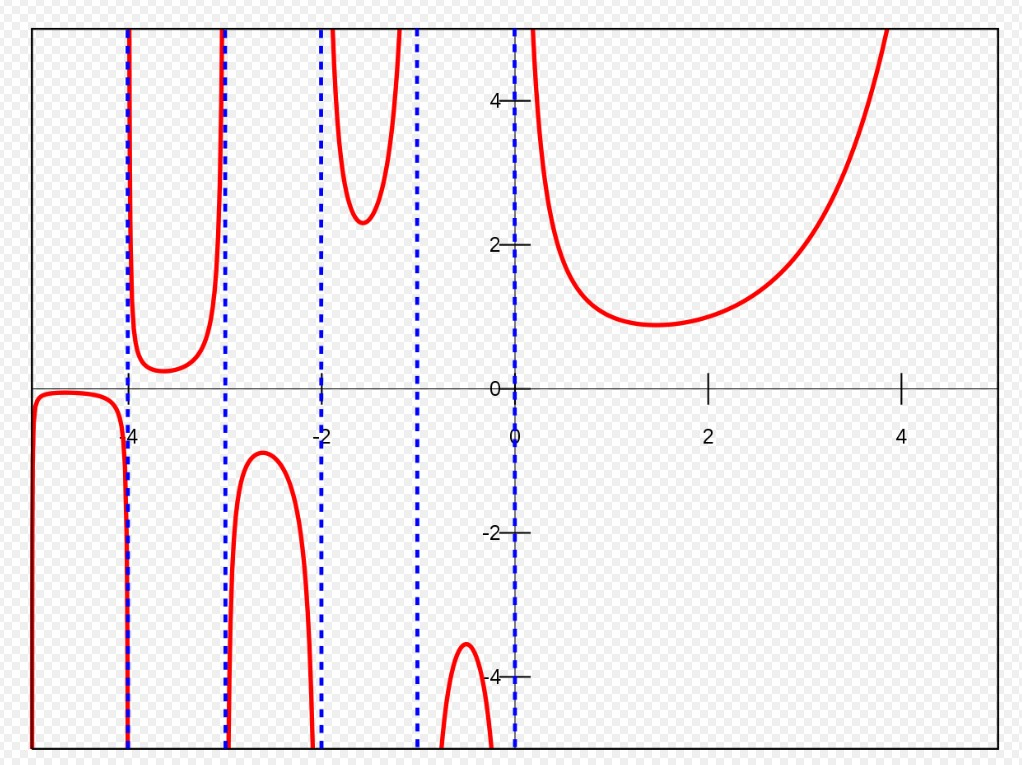
\includegraphics[width=0.5\textwidth]{gamma}
\end{figure}
\subsection{Stakeholders}
\begin{itemize}
\item User1: Mathematicians and researchers in the fields of calculus, mathematical analysis, statistics.
\item User2: Algorithm designers, researchers,engineers in the field of scientific computing in computer and software engineering.
\item User3: People with low maths and programming background who need to obtain the values of gamma function.
\item User4: 
\end{itemize}
\subsection{Domain}
All complex numbers except those whose real part are non-positive integers.
\\$$C/\{n\in Z, n\le 0\}$$
\subsection{Co-Domain}
All real numbers excluding zero.
\\$$\left ( -\infty,0  \right )\cup \left ( 0,+\infty  \right )$$
\subsection{Properties}
%https://en.wikipedia.org/wiki/Gamma_function#Properties
One of the important functional equatuations for the gamma fucntion is Euler's reflection formula:
\\$$\Gamma \left ( 1-z \right ) \Gamma \left ( z \right ) =\frac{\pi }{\sin \pi z},  z \notin Z $$ 
\\which implies,
\subsection{Perticular Values}
%https://en.wikipedia.org/wiki/Gamma_function#Particular_values
Including up to the first 20 digits after the decimal point, some of particular values of the gamma function are:
\begin{itemize}
\item $\Gamma \left ( -\frac{3}{2}  \right ) =\frac{4\sqrt{\pi } }{3} \approx +2.36327180120735470306$
\item $\Gamma \left ( -\frac{1}{2}  \right ) =-2\sqrt{\pi }  \approx -3.54490770181103205459$
\item $\Gamma \left ( \frac{1}{2}  \right ) =\sqrt{\pi }  \approx +1.77245385090551602729$
\item $\Gamma \left ( 1  \right ) =0! = +1$
\item $\Gamma \left ( \frac{3}{2}  \right ) =\frac{\pi }{2}   \approx +0.88622692545275801364$
\item $\Gamma \left ( 2 \right ) =1!=+1$
\item $\Gamma \left ( \frac{5}{2}  \right ) =\frac{3\sqrt{\pi } }{4} \approx +1.32934038817913702047$
\item $\Gamma \left ( 3  \right ) =2! \approx +2$
\item $\Gamma \left ( \frac{7}{2}   \right ) =\frac{15\sqrt{\pi } }{8}  \approx +3.32335097044784255118$
\item $\Gamma \left ( 4 \right ) =3!=+6$
\end{itemize}
\section{Requirements}
\subsection{Functional Requirements}
\begin{itemize}
\item FR1: We shall only consider the positive value as input value.
\item FR2: We shall only consider the real number as input value, ignore the imaginary part.
\item FR3: When the function value exceeds the maximum the value of a double type variable, the function will return NaN.
\end{itemize}
\subsection{Assumptions}

\section{Algorithm}
\subsection{Integrals Method}
\subsubsection{Description}
\subsubsection{Pseudocode}
\subsubsection{Advantages and Disadvantages}
\subsection{Lanczos Approximation}
\subsubsection{Description}
\subsubsection{Pseudocode}
\subsubsection{Advantages and Disadvantages}
\section{References}
But I don't want my section to be numbered. 
function = $\Gamma$
$\sqrt{1-\frac{v^2}{c^2}}$
\#\LaTeX\textbf{Rules}\!
\begin{itemize}
\item Item 1.
\item Item 2.
\item \ldots
\item Item n.
\end{itemize}
\begin{enumerate}
\item Item 1.
\item Item 2.
\item Item 3.
\end{enumerate}
\end{document}
